%----------------------------------------------------------------------------------------
%	PACKAGES AND OTHER DOCUMENT CONFIGURATIONS
%----------------------------------------------------------------------------------------

\documentclass[twoside,twocolumn]{article}

\usepackage{blindtext} % Package to generate dummy text throughout this template 
\usepackage{amsmath} % package for aligntment
\usepackage[sc]{mathpazo} % Use the Palatino font
\usepackage[T1]{fontenc} % Use 8-bit encoding that has 256 glyphs
\linespread{1.05} % Line spacing - Palatino needs more space between lines
\usepackage{microtype} % Slightly tweak font spacing for aesthetics
\usepackage{graphicx} % for pics 
\usepackage[english]{babel} % Language hyphenation and typographical rules

\usepackage[hmarginratio=1:1,top=32mm,columnsep=20pt]{geometry} % Document margins
\usepackage[hang, small,labelfont=bf,up,textfont=it,up]{caption} % Custom captions under/above floats in tables or figures
\usepackage{booktabs} % Horizontal rules in tables

\usepackage{lettrine} % The lettrine is the first enlarged letter at the beginning of the text

\usepackage{enumitem} % Customized lists
\setlist[itemize]{noitemsep} % Make itemize lists more compact

\usepackage{abstract} % Allows abstract customization
\renewcommand{\abstractnamefont}{\normalfont\bfseries} % Set the "Abstract" text to bold
\renewcommand{\abstracttextfont}{\normalfont\small\itshape} % Set the abstract itself to small italic text

\usepackage{titlesec} % Allows customization of titles
\renewcommand\thesection{\Roman{section}} % Roman numerals for the sections
\renewcommand\thesubsection{\roman{subsection}} % roman numerals for subsections
\titleformat{\section}[block]{\large\scshape\centering}{\thesection.}{1em}{} % Change the look of the section titles
\titleformat{\subsection}[block]{\large}{\thesubsection.}{1em}{} % Change the look of the section titles

\usepackage{fancyhdr} % Headers and footers
\pagestyle{fancy} % All pages have headers and footers
\fancyhead{} % Blank out the default header
\fancyfoot{} % Blank out the default footer
\fancyhead[C]{Goal Programming $\bullet$ May 2019 } % Custom header text
\fancyfoot[RO,LE]{\thepage} % Custom footer text

\usepackage{titling} % Customizing the title section

\usepackage{hyperref} % For hyperlinks in the PDF

%coding formatting
\usepackage{listings}
\usepackage{color}

\definecolor{dkgreen}{rgb}{0,0.6,0}
\definecolor{gray}{rgb}{0.5,0.5,0.5}
\definecolor{mauve}{rgb}{0.58,0,0.82}

\lstset{frame=tb,
  language=Python,
  aboveskip=3mm,
  belowskip=3mm,
  showstringspaces=false,
  columns=flexible,
  basicstyle={\small\ttfamily},
  numbers=none,
  numberstyle=\tiny\color{gray},
  keywordstyle=\color{blue},
  commentstyle=\color{dkgreen},
  stringstyle=\color{mauve},
  breaklines=true,
  breakatwhitespace=true,
  tabsize=3
}


%----------------------------------------------------------------------------------------
%	TITLE SECTION
%----------------------------------------------------------------------------------------

\setlength{\droptitle}{-4\baselineskip} % Move the title up

\pretitle{\begin{center}\Huge\bfseries} % Article title formatting
\posttitle{\end{center}} % Article title closing formatting
\title{Goal Programming} % Article title
\author{%
\textsc{Mirdha Suci Ananda, Yuda Hendriawan, Andi Aqil, Sumihar Christian}\thanks{A thank you or further information} \\[1ex] % Your name
\normalsize Department of Mathematical Computation and Data Science \\ % Your institution
\normalsize INSTITUT TEKNOLOGI SEPULUH NOPEMBER\\ % Your institution
}

\date{\today} % Leave empty to omit a date
\renewcommand{\maketitlehookd}{%
\begin{abstract}
\noindent Simulating Goal Programming on a product store sales problem with 3 types Goal Programming initiation method: Lexicographical, Weighted and Chebyshev using Pyomo for mathematical modelling in Python and GLPK for solving the optimization problem using simplex method
\end{abstract}
}

%----------------------------------------------------------------------------------------

\begin{document}

% Print the title
\maketitle

%----------------------------------------------------------------------------------------
%	ARTICLE CONTENTS
%----------------------------------------------------------------------------------------

\section{Introduction}

\lettrine[nindent=0em,lines=3]{O} rdinary linear program models are not able to solve management cases that require certain
goals to reach all objectives optimally at the same time. In the linear program model there
is a Slack variable in the constraint function in the form of a delimiter and a surplus in the
constraint function in the form of conditions. In solving the case of a linear program the two
variables function to accommodate the advantages and disadvantages of the left hand side value
of a constraint function so that it equals the value of the right hand side. However, both of
these variables are completely uncontrollable in solving the case of linear programs, so the linear
program model was developed by A. Charles and W. M. Cooper as a goal programming model.
If there are variables in a linear program that have characteristics similar to the Slack and
Surplus variables, and are in a constraint equation, then the variable is controlled so that the left
segment value of a constraint is equal to the value of the right segment. The goal programming
model is able to solve cases of linear programs that have more than one goal to be achieved.
The goal or target is a constant value on the right hand side of the constraint function
Basically the structure of goal programming and linear programming is the same. The
concept of goal programming is to introduce additional auxiliary variables called deviations
that act not as variable decision, but only as facilitators to formulate models. This deviation
is the difference between the desired target value and the results obtained.
The goal programming model is an extension of the linear program model so that all as-
sumptions, formation notations, mathematical models, formulation procedures, models and
solutions are no different. The difference lies only in

%------------------------------------------------

\section{General Form}
	Goal progamming is the one of the mathematical model used to make solution for the problem having many target so it can be got optimal solution. Aran Puntosadewo (2013) said that Goal Programming is for decising the goal notated by numerical for each goal, making objective function for each function, and finding solution to minimize the deviation at the objective function. Goal Programming model try to minimize the deviation between several goal or target, so the value of the right side is as close as possible to same with left side of the equation. 
	
	Goal Programming model is the extention of Linier Programming develoved by A. Charles and W. M Cooper at 1956 so all of the asumption, notation, mathematical formula, procuder of model and the solution are not different. The different of this program is just in the deviation exist in objective function and constraint. Linier Pogrmmiing is the mathematical model used to find the optimal solution with minimizing and maximizing objective function based on one constraint. Beside that, Goal Programming have three part, that is decision variable, objective function, and constraint.
	
	Having known that Goal Progamming have 3 part that are objective function, goal constraint, non negatif constraint. 
	\begin{itemize}
		\item[1. ] Objective Function\\
		Objective Function in Goal Programming basically is the problem of minimization, because at the objective function, there are deviation variable that has to minimize. Objective Function in the Goal Programming is for minimizing all of the goal constraint that want to be reached.
		
		\item[2. ] Non Negatif Constraint\\
		Non Negatif constraint in Goal Progamming is all of the variable that has positive value or equal to zero. So the decision variable and deviation variable at the Goal Programming problem always has positive value or equal to zero. The notation of non-negative is $x_j,d^-_i,d^+_i \geq 0$
		
		\item[3. ] Goal Constraint\\
		According to Rio Armindo (2006), at the Goal Programming, there are six kind of goal constraint different each other. The Goal from each constraint is decised by connection between objective function. this is the 6's kind of constraint.
	\end{itemize}
	
		\textbf{Common Model of Goal Programming}
		
		The first is the common model without priority factor in the structure :
		\begin{equation*}
		\text{Minimize}~~ Z = \displaystyle\sum_{i=1}^{m} \left(d^+_i + d^-_i\right)
		\end{equation*}
		with goal constraint :
		\begin{equation*}
		\begin{array}{rcl}
		C_{11}x_1+C_{12}x_2 + \dots + C_{1n}x_n + d^-_1 - d^+_1&=&b_1\\
		C_{21}x_1+C_{22}x_2 + \dots + C_{2n}x_n + d^-_2- d^+_2&=&b_2\\
		\vdots&&\\
		C_{m1}x_1+C_{m2}x_2 + \dots + C_{mn}x_n + d^-_m - d^+_m&=&b_m
		\end{array}
		\end{equation*}
		non negative constraint : $x_j,d^-_i,d^+_i \geq 0$, for $i = 1,2,\dots,m$ and $j = 1,2,\dots,n$
		
		\vspace{1cm}
		The Second is the problem at The Goal Programming with structur containing weight :
		\begin{equation*}
		\text{Minimize : }~~~ Z = P_1d^-_i + \dots + P_ld^-_i + P_{i+1}d^+_i +\dots + P_kd^+i
		\end{equation*}
		with constraint :
		\begin{equation*}
		\begin{array}{rcl}
		C_{11}x_1+C_{12}x_2 + \dots + C_{1n}x_n + d^-_1 - d^+_1&=&b_1\\
		C_{21}x_1+C_{22}x_2 + \dots + C_{2n}x_n + d^-_2- d^+_2&=&b_2\\
		\vdots&&\\
		C_{m1}x_1+C_{m2}x_2 + \dots + C_{mn}x_n + d^-_m - d^+_m&=&b_m
		\end{array}
		\end{equation*}
		Where $P_k$ is the weight of the goal -$k$
		and $$x_j,d^-_i,d^+_i \geq 0$$
		$P_k $ can be called by penalty for each goal, so if the goal is not same with sign in beginning, the goal will got penalty as much as $P_k$

\subsection{Weighted Goal Programming}		
The Second is the problem at The Goal Programming with structure containing weight :
		\begin{equation*}
		\text{Minimize : }~~~ Z = P_1d^-_i + \dots + P_ld^-_i + P_{i+1}d^+_i +\dots + P_kd^+i
		\end{equation*}
		with constraint :
		\begin{equation*}
		\begin{array}{rcl}
		C_{11}x_1+C_{12}x_2 + \dots + C_{1n}x_n + d^-_1 - d^+_1&=&b_1\\
		C_{21}x_1+C_{22}x_2 + \dots + C_{2n}x_n + d^-_2- d^+_2&=&b_2\\
		\vdots&&\\
		C_{m1}x_1+C_{m2}x_2 + \dots + C_{mn}x_n + d^-_m - d^+_m&=&b_m
		\end{array}
		\end{equation*}
		Where $P_k$ is the weight of the goal -$k$
		and $$x_j,d^-_i,d^+_i \geq 0$$
		$P_k $ can be called by penalty for each goal, so if the goal is not same with sign in beginning, the goal will got penalty as much as $P_k$
		
\subsection{Lexicographic Goal Programming}
		The second variant of a Goal Programming method presented in this section is called lexicographic Goal Programming. It can also be found in the literature as preemptive Goal Programming. The main feature of this variant is the existence of a number of priority levels. This variant is used when the decision maker has a clear preference order for satisfying the goals. Each priority level consists of a number of unwanted deviations to be minimized. We define by L the number of priority levels with corresponding index $l = 1, 2, \dots , L.$ Each priority level is a function of a subset of unwanted deviational variables, $h_l(n, p)$. The consensus in the goalprogramming literature is that no more than five priority levels should be used in this variant.
		
		A lexicographic Goal Programming problem can be represented by the following
		formulation
		$$\text{min }~z = h_1(n,p),h_2(n,p),\dots,h_L(n,p)$$
		$$\text{Subject to } f_i(x)+n_i+p_i=b_i~~,~~x\in F$$
		$$n_i,p_i \geq 0, i = 1,2,\dots,m$$
		
\subsection{Chebyshev Goal Programming}
The third variant of a Goal Programming method presented in this section is called
		Chebyshev Goal Programming. This variant was introduced by Flavell [6] and it is
		known as Chebyshev Goal Programming, because it uses the Chebyshev distance or L$\infty$ metric. It can also be found in the literature as Minmax Goal Programming. The main idea of this variant is to achieve a balance between the goals. Classical, weighted and lexicographic Goal Programming often find extreme solutions, i.e.,
		points that lie in the intersection of goals, constraints, and axes. This can lead to an unbalanced solution since some goals are achieved and others are far from satisfactory. In Chebyshev Goal Programming, we introduce additional constraints in order to ensure balance between the goals. This is the only widely-used variant that can find optimal solutions that are not located at extreme points.
		
		Let $\lambda$ be the maximal deviation from amongst the set of goals, then a generic
		form of a Chebyshev Goal Programming problem is the following
		

\begin{align}
		\text{min } ~ z &= \lambda \\
		\text{s.t. } \dfrac{u_in_i}{k_i}+\dfrac{v_ip_i}{k_i} + &\leq \lambda \\
		f_i(x)+n_i+p_i &= b_i~~~~, x\in F \\
		n_i,p_i \geq 0, i = 1,2,\dots,m \\
\end{align}
%------------------------------------------------

\section{Problem}
A store produces and sells shirts and jackets. The price of a shirt is at 100 e, while the price of a jacket is at 90 Euro. Every shirt needs 2 $m^2$ of cotton and 5 $m^2$ of linen, while every jacket needs 4 $m^2$ of cotton and 3 $m^2$ of linen. The store can buy from its supplier 600 $m^2$ of cotton and 700 $m^2$ of linen every week. The company aims to achieve a weekly profit of 18,000 Euro. The production time of a pair of each product is 2 man-hours. The company employs 10 people in the production department and would like to keep within the 380 available hours of work each week. The manufacturing capacity of the machine for all products combined is limited to a maximum of 200 products per week. The company has signed a contract with a customer to provide his/her company with at least 60 units of each product per week.

\subsection{Variables}
$x_1 = $ number of shirts, \\
$x_2 = $ number of jackets\\

\subsection{Constraints}
\begin{align}
2x_1 + 4x_2 \leq 600 Cotton  Stock \\
5x_1 + 3x_2 \leq 700 Linen Stock \\
100x_1 + 90x_2 \geq 18000 Weekly Profit minimum \\
2x_1 + 2x_2 \leq 380 Man-hours available \\
x_1 + x_2 \leq 200 Machine Limitation \\
x_1,x_2 \geq 60 Minimum Production's Contract 
\end{align}

\subsection{Modelling}
So we can formulate the problem into goal programming: 
\begin{center}
   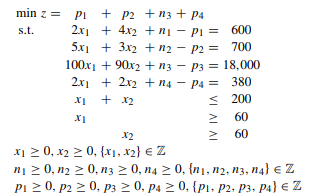
\includegraphics[scale=0.6]{/home/svmihar/Documents/kuliah/ro2/project_goal_optimization/prob.png}
\end{center}

By drawing a plane from the problem we know that it has no possible solution 
\begin{figure}[h]
  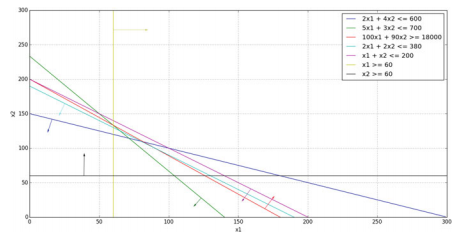
\includegraphics[scale=0.5]{/home/svmihar/Documents/kuliah/ro2/project_goal_optimization/infeasible.png}
  \caption{no feasible region}
  \label{fig:boat1}
\end{figure}

%------------------------------------------------

\section{Methods}

\subsection{Lexicographical}

Lexicographical Goal Programming use priority levels for each goals. The linear program will run separately for each priority level, running in sequence of order from the highest to lowest priority. \\
\\
This will be the priority level for each of the goals :
\begin{description}
  \item[$\bullet$ Priority Level 1] Man-hours (Goal 4)
  \item[$\bullet$ Priority Level 2] Weekly Profit (Goal 3)
  \item[$\bullet$ Priority Level 3] Cotton and Linen stocks to buy (Goal 1 and Goal 2)
\end{description}

The first linear program is to solve Priority Level 1, which is to minimize man hour excess.
\\
\\
\textbf{Priority Level 1 LP}\\
$Minimize \ d_4^{+}$ \\
$Subject \ to$
\begin{align*}
2x_1 + 4x_2 + d_1^{-} - d_1^{+} &= 600\\
5x_1 + 3x_2 + d_2^{-} - d_2^{+} &= 700\\
100x_1 + 90x_2 + d_3^{-} - d_3^{+} &= 18000\\
2x_1 + 2x_2 + d_4^{-} - d_4^{+} &= 600 \\
x_1 + x_2 &\leq 200 \\
x_1, x_2 &\geq 60 \\
d_1^{-}, d_1^{+}, d_2^{-}, d_2^{+}, d_3^{-}, d_3^{+}, d_4^{-}, d_4^{+} &\geq 0
\end{align*}

This linear program can be solved using any method such as Simplex Method, Graphical Method or using any Solver. The results we get is $d_4^{+} = 0$ which fully satisfy the goal. \\

The idea is to use the previous results for the next priority goal we want to accomplish. We will use the results from first Linear Program as a constraints for the next one. The second Linear Program is to achieve weekly profit.\\
\\
\textbf{Priority Level 2 LP}\\
$Minimize \ d_3^{-}$ \\
$Subject \ to$
\begin{align*}
2x_1 + 4x_2 + d_1^{-} - d_1^{+} &= 600\\
5x_1 + 3x_2 + d_2^{-} - d_2^{+} &= 700\\
100x_1 + 90x_2 + d_3^{-} - d_3^{+} &= 18000\\
2x_1 + 2x_2 + d_4^{-} - d_4^{+} &= 600 \\
d_4^{+} &= 0 \\
x_1 + x_2 &\leq 200 \\
x_1, x_2 &\geq 60 \\
d_1^{-}, d_1^{+}, d_2^{-}, d_2^{+}, d_3^{-}, d_3^{+}, d_4^{-}, d_4^{+} &\geq 0 
\end{align*}

The results we get from the second Linear Program is $d_3^{-} = 0$ which fully satisfy the second level priority goal. \\

The third Linear Program will use the second Linear Program's constraints and its results. \\
\\
\textbf{Priority Level 3 LP}\\
$Minimize \ d_1^{+} + d_2^{+}$ \\
$Subject \ to$
\begin{align*}
2x_1 + 4x_2 + d_1^{-} - d_1^{+} &= 600\\
5x_1 + 3x_2 + d_2^{-} - d_2^{+} &= 700\\
100x_1 + 90x_2 + d_3^{-} - d_3^{+} &= 18000\\
2x_1 + 2x_2 + d_4^{-} - d_4^{+} &= 600 \\
d_4^{+} &= 0 \\
d_3^{-} &= 0  \\
x_1 + x_2 &\leq 200 \\
x_1, x_2 &\geq 60 \\
d_1^{-}, d_1^{+}, d_2^{-}, d_2^{+}, d_3^{-}, d_3^{+}, d_4^{-}, d_4^{+} &\geq 0 
\end{align*}
The result for this linear program is $d_1^{+} = 0$, $d_1^{-} = 20$, $d_2^{+} = 50$ and $d_2^{-} = 0$ \\

This will be the final results :
\begin{align*}
x_1 &= 90 \\
x_2 &= 100 \\
d_1^{+} &= 0, \ d_1^{-} = 20 \\
d_2^{+} &= 50, d_2^{-} = 0 \\
d_3^{+} &= 0, \ d_3^{-} = 0 \\
d_4^{+} &= 0, \ d_4^{-} = 0 
\end{align*}

\begin{lstlisting}
// Lexicograhical.py
# first priority level
model.obj = Objective(expr = model.p4)

# Define the constraints
model.con1 = Constraint(expr = 2 * model.x1 +
    4 * model.x2 + model.n1 - model.p1 == 600)
model.con2 = Constraint(expr = 5 * model.x1 +
    3 * model.x2 + model.n2 - model.p2 == 700)
model.con3 = Constraint(expr = 100 * model.x1 +
    90 * model.x2 + model.n3 - model.p3 == 18000)
model.con4 = Constraint(expr = 2 * model.x1 +
    2 * model.x2 + model.n4 - model.p4 == 380)
model.con5 = Constraint(expr = model.x1 +
    model.x2 <= 200)
model.con6 = Constraint(expr = model.x1 >= 60)
model.con7 = Constraint(expr = model.x2 >= 60)

# Solve the Goal Programming problem of the
# first priority level
opt.solve(model)

# Retrieve the value of the first priority level
p4 = model.p4.value

# Define the objective function of the
# second priority level
model.obj = Objective(expr = model.n3)

# Add a constraint for the value of the first
# priority level
model.con8 = Constraint(expr = model.p4 == p4)

# Solve the Goal Programming problem of the
# second priority level
opt.solve(model)

# Retrieve the value of the second priority level
n3 = model.n3.value

# Define the objective function of the
# third priority level
model.obj = Objective(expr = model.p1 + model.p2)

# Add a constraint for the value of the second
# priority level
model.con9 = Constraint(expr = model.n3 == n3)

# Solve the Goal Programming problem of the
# third priority level
opt.solve(model)

# Print the values of the decision variables
print("x1 = ", model.x1.value)
print("x2 = ", model.x2.value)

# Print the achieved values for each goal
if model.n1.value > 0:
    print("The first goal is underachieved by ",
          model.n1.value)
elif model.p1.value > 0:
    print("The first goal is overachieved by ",
          model.p1.value)
else:
    print("The first goal is fully satisfied")

if model.n2.value > 0:
    print("The second goal is underachieved by ",
          model.n2.value)
elif model.p2.value > 0:
    print("The second goal is overachieved by ",
          model.p2.value)
else:
    print("The second goal is fully satisfied")

if model.n3.value > 0:
    print("The third goal is underachieved by ",
          model.n3.value)
elif model.p3.value > 0:
    print("The third goal is overachieved by ",
          model.p3.value)
else:
    print("The third goal is fully satisfied")

if model.n4.value > 0:
    print("The fourth goal is underachieved by ",
          model.n4.value)
elif model.p4.value > 0:
    print("The fourth goal is overachieved by ",
          model.p4.value)
else:
    print("The fourth goal is fully satisfied")
\end{lstlisting}


\subsection{Weighted}

\blindtext % Dummy text

\begin{lstlisting}
model.obj = Objective(expr = (1 / 600) * model.p1 +
    (1 / 700) * model.p2 + (2 / 18000) * model.n3 +
    (3 / 380) * model.p4)

# Define the constraints
model.con1 = Constraint(expr = 2 * model.x1 +
    4 * model.x2 + model.n1 - model.p1 == 600)
model.con2 = Constraint(expr = 5 * model.x1 +
    3 * model.x2 + model.n2 - model.p2 == 700)
model.con3 = Constraint(expr = 100 * model.x1 +
    90 * model.x2 + model.n3 - model.p3 == 18000)
model.con4 = Constraint(expr = 2 * model.x1 +
    2 * model.x2 + model.n4 - model.p4 == 380)
model.con5 = Constraint(expr = model.x1 +
    model.x2 <= 200)
model.con6 = Constraint(expr = model.x1 >= 60)
model.con7 = Constraint(expr = model.x2 >= 60)

# Solve the Goal Programming problem
opt.solve(model)

# Print the values of the decision variables
print("x1 = ", model.x1.value)
print("x2 = ", model.x2.value)

# Print the achieved values for each goal
if model.n1.value > 0:
    print("The first goal is underachieved by ",
          model.n1.value)
elif model.p1.value > 0:
    print("The first goal is overachieved by ",
          model.p1.value)
else:
    print("The first goal is fully satisfied")

if model.n2.value > 0:
    print("The second goal is underachieved by ",
          model.n2.value)
elif model.p2.value > 0:
    print("The second goal is overachieved by ",
          model.p2.value)
else:
    print("The second goal is fully satisfied")

if model.n3.value > 0:
    print("The third goal is underachieved by ",
          model.n3.value)
elif model.p3.value > 0:
    print("The third goal is overachieved by ",
          model.p3.value)
else:
    print("The third goal is fully satisfied")

if model.n4.value > 0:
    print("The fourth goal is underachieved by ",
          model.n4.value)
elif model.p4.value > 0:
    print("The fourth goal is overachieved by ",
          model.p4.value)
else:
    print("The fourth goal is fully satisfied")
\end{lstlisting}



\subsection{Chebyshev}

\begin{enumerate}
	\item Determine whether a constraint is soft or hard.
	\item Add a negative and a positive deviational variable on each constraint. Determine the type of the constraint and add a constraint of the deviational variable(s) to be penalized. For each deviational variable, select a weight. 
	\item Use a normalization method to scale the deviations.
	\item Each hard constraint is written as a typical linear programming constraint.
	\item Add bound constraints to the problem (if applicable).
\end{enumerate}
\begin{lstlisting}
# Define the decision variables
model.x1 = Var(within = NonNegativeIntegers)
model.x2 = Var(within = NonNegativeIntegers)

# Define the deviational variables
model.n1 = Var(within = NonNegativeIntegers)
model.p1 = Var(within = NonNegativeIntegers)
model.n2 = Var(within = NonNegativeIntegers)
model.p2 = Var(within = NonNegativeIntegers)
model.n3 = Var(within = NonNegativeIntegers)
model.p3 = Var(within = NonNegativeIntegers)
model.n4 = Var(within = NonNegativeIntegers)
model.p4 = Var(within = NonNegativeIntegers)

# Define the variable of maximal deviation
# from amongst the set of goals
model.l = Var(within=NonNegativeReals)

# Define the objective function
model.obj = Objective(expr = model.l)

# Define the constraints
model.con1 = Constraint(expr = (1 / 600) *
    model.p1 <= model.l)
model.con2 = Constraint(expr = (1 / 700) *
    model.p2 <= model.l)
model.con3 = Constraint(expr = (2 / 18000) *
    model.n3 <= model.l)
model.con4 = Constraint(expr = (3 / 380) *
    model.p4 <= model.l)
model.con5 = Constraint(expr = 2 * model.x1 +
    4 * model.x2 + model.n1 - model.p1 == 600)
model.con6 = Constraint(expr = 5 * model.x1 +
    3 * model.x2 + model.n2 - model.p2 == 700)
model.con7 = Constraint(expr = 100 * model.x1 +
    90 * model.x2 + model.n3 - model.p3 == 18000)
model.con8 = Constraint(expr = 2 * model.x1 +
    2 * model.x2 + model.n4 - model.p4 == 380)
model.con9 = Constraint(expr = model.x1 +
    model.x2 <= 200)
model.con10 = Constraint(expr = model.x1 >= 60)
model.con11 = Constraint(expr = model.x2 >= 60)

# Solve the Goal Programming problem
opt.solve(model)

# Print the values of the decision variables
print("x1 = ", model.x1.value)
print("x2 = ", model.x2.value)

# Print the achieved values for each goal
if model.n1.value > 0:
    print("The first goal is underachieved by ",
          model.n1.value)
elif model.p1.value > 0:
    print("The first goal is overachieved by ",
          model.p1.value)
else:
    print("The first goal is fully satisfied")

if model.n2.value > 0:
    print("The second goal is underachieved by ",
          model.n2.value)
elif model.p2.value > 0:
    print("The second goal is overachieved by ",
          model.p2.value)
else:
    print("The second goal is fully satisfied")

if model.n3.value > 0:
    print("The third goal is underachieved by ",
          model.n3.value)
elif model.p3.value > 0:
    print("The third goal is overachieved by ",
          model.p3.value)
else:
    print("The third goal is fully satisfied")

if model.n4.value > 0:
    print("The fourth goal is underachieved by ",
          model.n4.value)
elif model.p4.value > 0:
    print("The fourth goal is overachieved by ",
          model.p4.value)
else:
    print("The fourth goal is fully satisfied")
\end{lstlisting}

%------------------------------------------------

\section{Results}

\begin{table}[h]
\caption{Solution for Lexicographical}
\centering
\begin{tabular}{lllr}
Goal & Target & Achieved Value \\
\midrule
1    & 600    & 580            \\ 
2    & 700    & 750            \\ 
3    & 18000  & 18000          \\ 
4    & 380    & 380            \\ 
\bottomrule
\end{tabular}
\end{table}

\begin{table}[h]
\caption{Solution for Weighted}
\centering
\begin{tabular}{lllr}
Goal & Target & Achieved Value \\
\midrule
1    & 600    & 614 \\ 
2    & 700    & 716            \\ 
3    & 18000  & 17830 \\ 
4    & 380    & 380            \\ 
\bottomrule
\end{tabular}
\end{table}

\begin{table}[h]
\caption{Solution for Chebyshev}
\centering
\begin{tabular}{lllr}
Goal & Target & Achieved Value \\
\midrule
1    & 600    & 614            \\ 
2    & 700    & 716            \\ 
3    & 18000  & 17830 			\\ 
4    & 380    & 380            \\ 
\bottomrule
\end{tabular}
\end{table}

From the result we have Chebyshev that has most balanced solution
\pagebreak
%----------------------------------------------------------------------------------------
%	REFERENCE LIST
%----------------------------------------------------------------------------------------
\begin{thebibliography}{99} % Bibliography - this is intentionally simple in this template 
 
\bibitem[Marc J. Schniederjans, 1995]{asdf:asdf}
Marc J. Schniederjans. ~A. (1995).
\newblock Goal Programming Methodology and Applications - a cross-cultural
  study.
\newblock {\em Goal Programming}, 20:317--330.


\bibitem[Papathanasiou and Ploskas, 2017]{Figueredo:2009dg}
Papathanasiou , ~J. and Ploskas, ~N. (2017).
\newblock Multiple Criteria Decision Aid. Methods, Examples and Python Implementations - a cross-cultural
  study.
\newblock {\em Goal Programming Numerical}, 20:317--330.
% Jason Papathanasiou, Nikolaos Ploskas - Multiple Criteria Decision Aid. Methods, Examples and Python Implementations (2018, Springer)


\bibitem[Papathanasiou and Ploskas, 2017]{Figueredo:2009dg}
Papathanasiou , ~J. and Ploskas, ~N. (2017).
\newblock Multiple Criteria Decision Aid. Methods, Examples and Python Implementations - a cross-cultural
  study.
\newblock {\em Goal Programming Numerical}, 20:317--330.
% Jason Papathanasiou, Nikolaos Ploskas - Multiple Criteria Deci

\bibitem[Papathanasiou and Ploskas, 2017]{Figueredo:2009dg}
Papathanasiou , ~J. and Ploskas, ~N. (2017).
\newblock Multiple Criteria Decision Aid. Methods, Examples and Python Implementations - a cross-cultural
  study.
\newblock {\em Goal Programming Numerical}, 20:317--330.
% Jason Papathanasiou, Nikolaos Ploskas - Multiple Criteria Deci

\end{thebibliography}

%----------------------------------------------------------------------------------------

\end{document}
